% TPOC-LPA (baseline) architecture flowchart, moved out of the paper. Compile: tectonic tpoc_lpa_baseline_architecture.tex
% Caption used in the paper: Architecture of the baseline TPOC-LPA~(Kong et al., 2026). Oval = start/end, parallelogram = input/output, rectangle = process, diamond = decision.
\documentclass[border=6pt]{standalone}
\usepackage{amsmath,amssymb}
\DeclareMathOperator*{\argmax}{arg\,max}
\usepackage{tikz}
\usetikzlibrary{shapes.geometric,shapes.misc,arrows.meta,positioning,fit,backgrounds,calc}
\tikzset{
  term/.style={rounded rectangle, draw, thick, font=\scriptsize, minimum height=5mm, minimum width=12mm, fill=gray!12},
  io/.style={trapezium, trapezium left angle=72, trapezium right angle=108, draw, thick, font=\scriptsize, align=center, minimum height=6.5mm, fill=gray!8},
  proc/.style={rectangle, draw, thick, font=\scriptsize, align=center, minimum height=7mm, inner sep=2.5pt},
  dec/.style={diamond, aspect=2.4, draw, thick, font=\scriptsize, align=center, inner sep=1.5pt},
  newp/.style={proc, fill=blue!14},
  modp/.style={proc, fill=orange!28},
  arr/.style={-{Stealth[length=1.8mm,width=1.5mm]}, thick},
  lab/.style={font=\scriptsize\itshape, inner sep=1pt}
}
\begin{document}
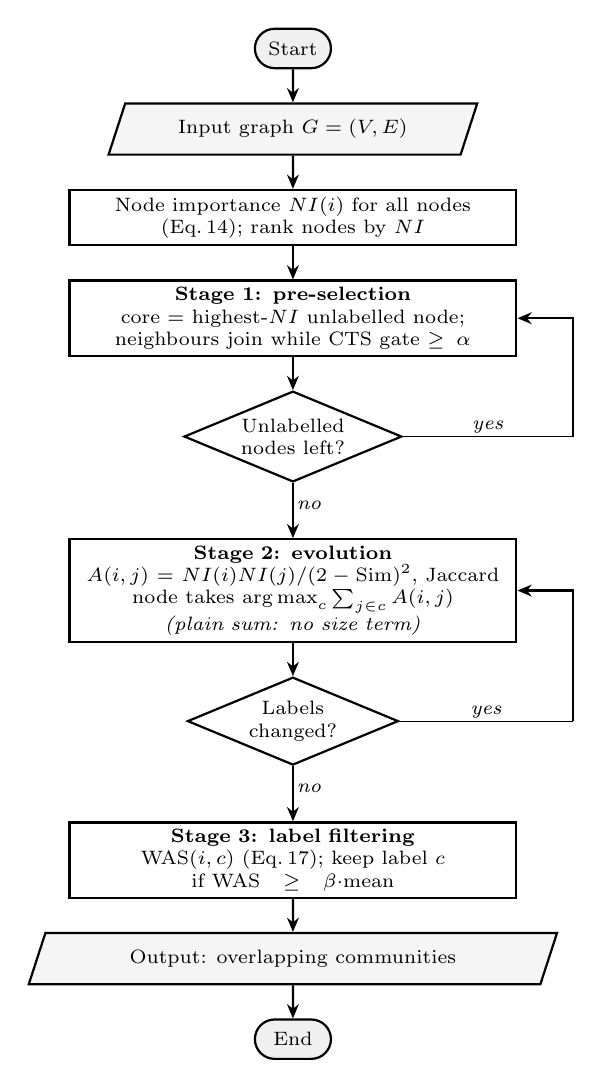
\begin{tikzpicture}[node distance=4.2mm]
\node[term] (s) {Start};
\node[io, below=of s] (in) {Input graph $G=(V,E)$};
\node[proc, below=of in, text width=55mm] (ni) {Node importance $NI(i)$ for all nodes\\(Eq.\,14); rank nodes by $NI$};
\node[proc, below=of ni, text width=55mm] (s1) {\textbf{Stage 1: pre-selection}\\ core = highest-$NI$ unlabelled node;\\ neighbours join while CTS gate $\ge\alpha$};
\node[dec, below=of s1] (d1) {Unlabelled\\nodes left?};
\node[proc, below=7mm of d1, text width=55mm] (s2) {\textbf{Stage 2: evolution}\\ $A(i,j)=NI(i)NI(j)/(2-\mathrm{Sim})^2$, Jaccard\\ node takes $\argmax_c\sum_{j\in c}A(i,j)$\\ \textit{(plain sum: no size term)}};
\node[dec, below=of s2] (d2) {Labels\\changed?};
\node[proc, below=7mm of d2, text width=55mm] (s3) {\textbf{Stage 3: label filtering}\\ $\mathrm{WAS}(i,c)$ (Eq.\,17); keep label $c$\\ if $\mathrm{WAS}\ge\beta\cdot$mean};
\node[io, below=of s3] (out) {Output: overlapping communities};
\node[term, below=of out] (e) {End};
\draw[arr] (s)--(in); \draw[arr] (in)--(ni); \draw[arr] (ni)--(s1); \draw[arr] (s1)--(d1);
\draw[arr] (d1)--(s2) node[lab, pos=.4, right]{no};
\coordinate (p1) at ($(d1.east -| s1.east)+(7mm,0)$);
\draw (d1.east) -- (p1) node[lab, pos=.5, above]{yes};
\draw[arr] (p1) -- (p1 |- s1.east) -- (s1.east);
\draw[arr] (s2)--(d2);
\draw[arr] (d2)--(s3) node[lab, pos=.4, right]{no};
\coordinate (p2) at ($(d2.east -| s2.east)+(7mm,0)$);
\draw (d2.east) -- (p2) node[lab, pos=.5, above]{yes};
\draw[arr] (p2) -- (p2 |- s2.east) -- (s2.east);
\draw[arr] (s3)--(out); \draw[arr] (out)--(e);
\end{tikzpicture}
\end{document}
